\chapter{Description of Recorded Signals}



\begin{center}
\begin{longtable}{c c c c} 
 \toprule
 Signal & Sensor & Frequency & Samples \\ [0.5ex] 
 \midrule
 C:s ist/X & TNC Scope & 10 kHz & 75000 \\ 

 C:s soll/X & TNC Scope & 10 kHz & 75000 \\ 

 C:s diff/X & TNC Scope & 10 kHz & 75000 \\ 

 C:v (n ist)/X & TNC Scope & 10 kHz & 75000 \\ 

 C:v (n soll)/X& TNC Scope & 10 kHz & 75000 \\ 

 C:P mech./X & TNC Scope & 10 kHz & 75000 \\ 

 C:Pos. Diff./X & TNC Scope & 10 kHz & 75000 \\ 

 C:I ist/X & TNC Scope & 10 kHz & 75000 \\ 

 C:I soll/X & TNC Scope & 10 kHz & 75000 \\ 

 C:x bottom & Acc & 10 kHz & 75000 \\ 

 C:y bottom & Acc & 10 kHz & 75000 \\ 

 C:z bottom & Acc & 10 kHz & 75000 \\ 

 C:x nut & Acc & 10 kHz & 75000 \\ 

 C:y nut & Acc & 10 kHz & 75000 \\ 

 C:z nut & Acc & 10 kHz & 75000 \\ 

 C:x top & Acc & 10 kHz & 75000 \\ 

 C:y top & Acc & 10 kHz & 75000 \\ 

 C:z top & Acc & 10 kHz & 75000 \\ 

 D:s ist/X & TNC Scope & 10 kHz & 75000 \\

 D:s soll/X & TNC Scope & 10 kHz & 75000 \\ 

 D:s diff/X & TNC Scope & 10 kHz & 75000 \\ 

 D:v (n ist)/X & TNC Scope & 10 kHz & 75000 \\ 

 D:v (n soll)/X & TNC Scope & 10 kHz & 75000 \\ 

 D:P mech./X & TNC Scope & 10 kHz & 75000 \\ 
 
 D:Pos. Diff./X & TNC Scope & 10 kHz & 75000 \\ 

 D:I ist/X & TNC Scope & 10 kHz & 75000 \\ 

 D:I soll/X & TNC Scope & 10 kHz & 75000 \\ 

 D:x bottom & Acc & 10 kHz & 75000 \\ 

 D:y bottom & Acc & 10 kHz & 75000 \\ 

 D:z bottom & Acc & 10 kHz & 75000 \\ 

 D:x nut & Acc & 10 kHz & 75000 \\ 

 D:y nut & Acc & 10 kHz & 75000 \\ 

 D:z nut & Acc & 10 kHz & 75000 \\ 

 D:x top & Acc & 10 kHz & 75000 \\

 D:y top & Acc & 10 kHz & 75000 \\ 

 D:z top & Acc & 10 kHz & 75000 \\ 

 S:x bottom & Acc & 10 kHz & 153601 \\ 

 S:y bottom & Acc & 10 kHz & 153601 \\ 

 S:z bottom & Acc & 10 kHz & 153601 \\ 

 S:x nut & Acc & 10 kHz & 153601 \\ 

 S:y nut & Acc & 10 kHz & 153601 \\ 

 S:z nut & Acc & 10 kHz & 153601 \\ 

 S:x top & Acc & 10 kHz & 153601 \\ 

 S:y top & Acc & 10 kHz & 153601 \\ 
 
 S:z top & Acc & 10 kHz & 153601 \\ 
 
 S:Nominal rotational speed & TNC opt & 1 kHz & 16384 \\
 
 S:Actual rotational speed & TNC opt & 1 kHz & 16384 \\ 
 
 S:Actual position of the position encoder(dy/dt) & TNC opt & 1 kHz & 16384 \\ 
 S:Actual position of the motor encoder(dy/dt)  & TNC opt & 1 kHz & 16384  \\ [1ex] 
 \bottomrule
\caption {Description of recorded signals}
\label {tab:description_of_the_49_recorded_features}
\end{longtable}
\end{center}


\begin{comment}
    

If there are several additions you want to add, but they do not fit into the thesis itself, they belong here.


\section{Generative Adversarial Network}
Generative Adversarial Networks (GANs) are generative models which recently became more and more popular. Generative models can capture the data distribution of samples seen during training. Such models are able to synthetically generate new instances belonging to the train data distribution without actually being part of that dataset. They can be used in an unsupervised or a supervised manner, which means, they are able to perform feature learning/extraction and classification. GANs include two different models. A generator network (G) learns the data distribution of the training data. Given noise, the generator network produces synthetic data. The discriminator (D) model tries to classify the seen data between synthetic generator's output and true data. D(x) represents the probability that x comes from the real data rather than from the generator. The optimization process of GANs is a minimax game process:
\begin{equation}
    \min_{G} \max_{D} \mathbb{E}_{x \sim P_{r}} [log(D(x))] + \mathbb{E}_{\tilde{x} \sim P_{g}}[log(1-D(\tilde{x}))],
    \label{eq:GAN_Training}
\end{equation}
where $P_{r}$ is the distribution of the real input data and $P_{g}$ is the data distribution from the generator's output, which is defined by  $\tilde{x}  \sim G(z)$. A Uniform or Gaussian distribution can be used to sample the noise $z \sim p(z)$. In theory the generator should be learned such that eq. \ref{eq:GAN_Training} is minimized. This is achieved if the discriminator falsely classifies the real and the synthetic generator's outputs ($D(x) \sim 0$ and $D(\tilde{x}) \sim 1$). On the other hand, the discriminator should be learned such that eq. \ref{eq:GAN_Training} is maximized, which means that the discriminator correctly labels all samples ($D(x) \sim 1$ and $D(\tilde{x}) \sim 0$). The discriminator and generator are optimized in an alternating procedure \cite{Goodfellow2014}. In order to prevent overfitting, one should alternate between k steps of optimizing D and one step of optimizing G \cite{Goodfellow2014}. The optimization of GANs proposed by Goodfellow et al \cite{Goodfellow2014} is described in the Algorithm \ref{alg.GAN_optimization}.

\begin{algorithm}
\caption{Iterative optimization of GANs}\label{alg:cap}
\begin{algorithmic}
\While{$\textrm{train iterations} < \textrm{max iterations}$}
    \While{$\textrm{discriminator optimization steps} < \textrm{k}$}
        \State $\cdot$ Sample m noise samples ${\pmb{z}^{(1)}, . . . , \pmb{z}^{(m)}}$ from noise distribution $p(\pmb{z})$
        \State $\cdot$ Sample m noise samples ${\pmb{x}^{(1)}, . . . , \pmb{x}^{(m)}}$ from real data distribution $P_{r}$
        \State $\cdot$ Update the discriminator by ascending its stochastic gradient:
        \begin{equation*}
            \nabla_{\theta_{d}} \frac{1}{m} \sum_{i=1}^{m} [log(D(\pmb{x}^{(i)})) + log(1-D(G(\pmb{z}^{(i)})))].
        \end{equation*}
    \EndWhile
    \State $\cdot$ Sample m noise samples ${\pmb{z}^{(1)}, . . . , \pmb{z}^{(m)}}$ from noise distribution $p(\pmb{z})$
    \State $\cdot$ Update the generator by descending its stochastic gradient:
    \begin{equation*}
        \nabla_{\theta_{g}} \frac{1}{m} \sum_{i=1}^{m} log(1-D(G(\pmb{z}^{(i)}))).
    \end{equation*}
\EndWhile
\label{alg.GAN_optimization}
\end{algorithmic}
\end{algorithm}

Besides that, eq. \ref{eq:GAN_Training} does not deliver sufficient gradients for gradient-based optimization of GANs. The problem is, that in early stages the generator performance is poor, such that the discriminator rejects all synthetic generator's outputs, which prevents the generator training. Instead, the generator can be trained to maximize $D(\tilde{x})$. This objective achieves the same results as eq. \ref{eq:GAN_Training} but delivers stronger gradients in early learning stages \cite{Goodfellow2014}. Fig \ref{fig:GAN_training_vizualization} shows the alternating optimization of the discriminator and generator. 

\begin{figure}[H]
  \centering
  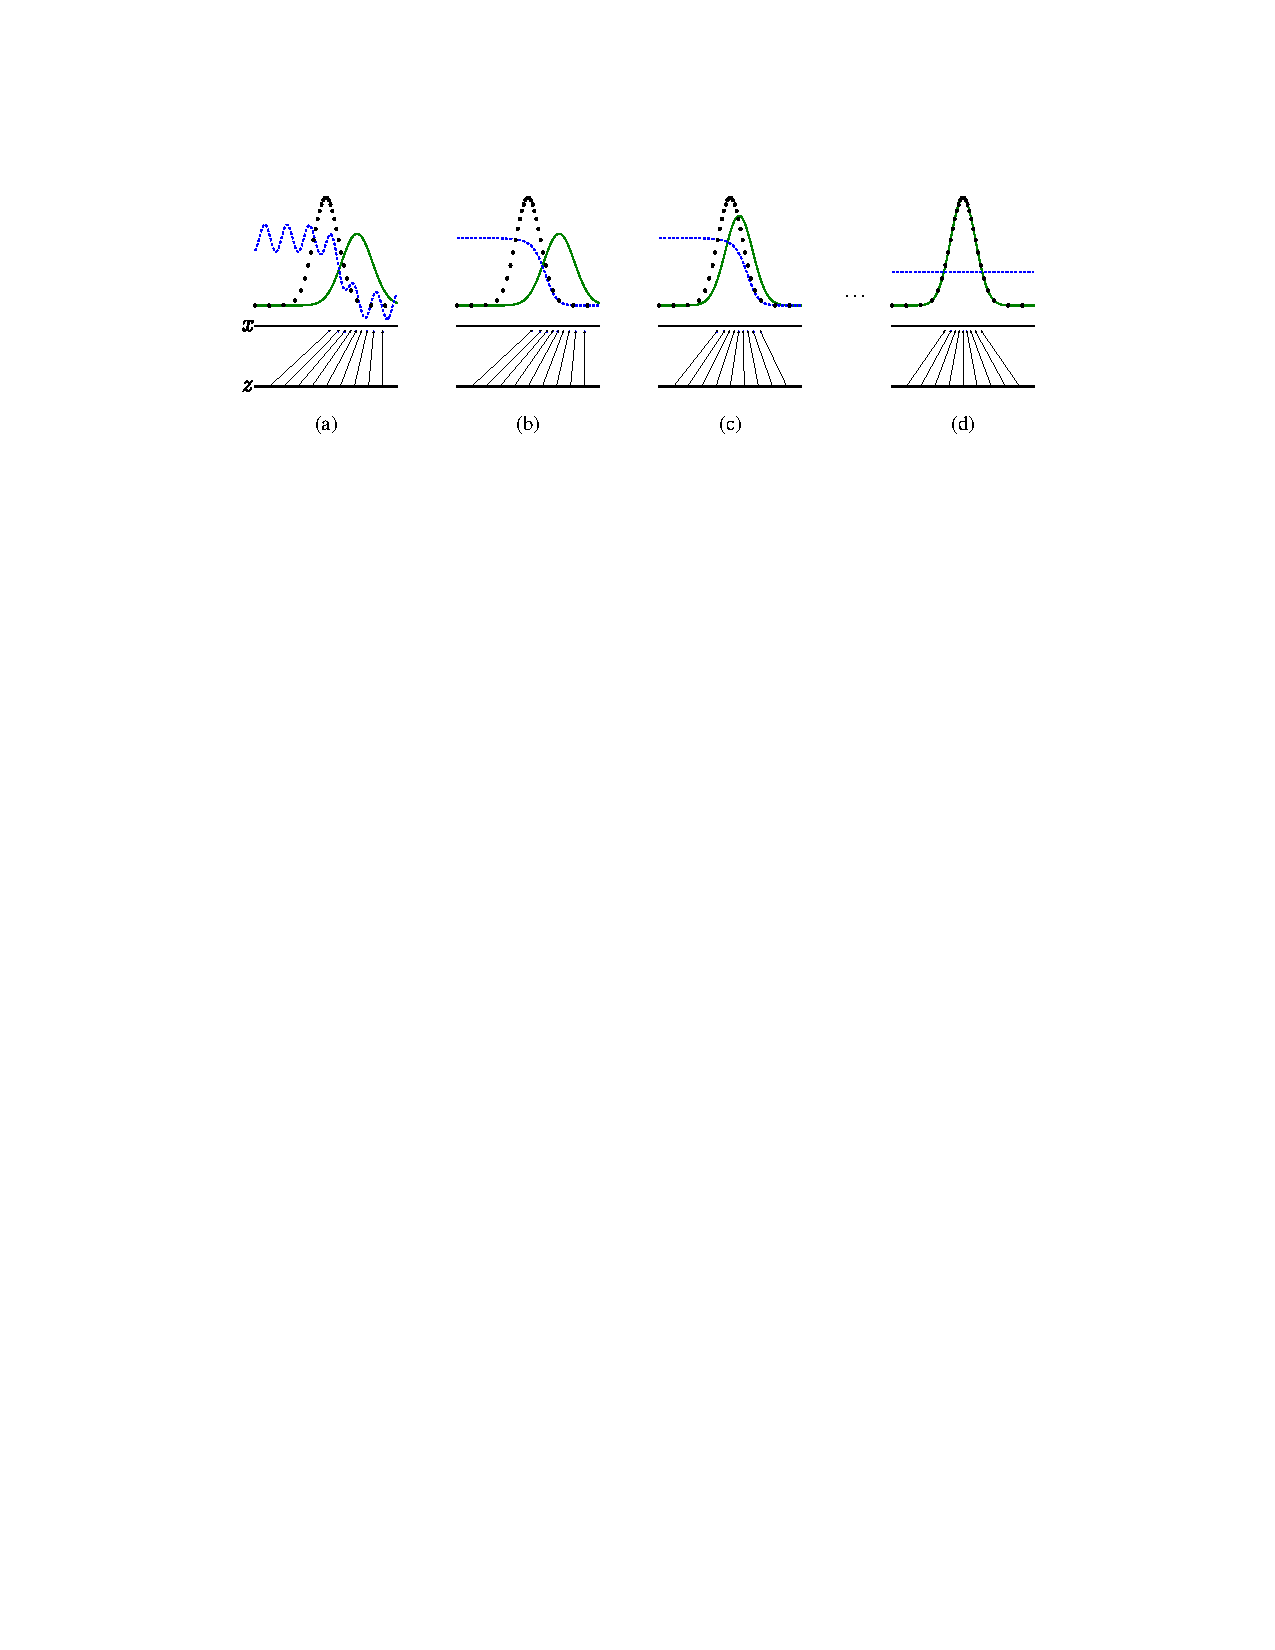
\includegraphics[width=1\textwidth]{GAN_training_vizualization.pdf}
  \caption{When optimizing GANs the discriminator and generator are optimized simultaneously in an alternating procedure. The blue dashed line represents the discriminator probability of x belonging to the real data distribution rather than being created by the generator. The black dashed line represents the generative distribution and the green solid line the real data distribution. (a) shows a generator, discriminator pair near convergence, (b) shows the GAN performance after passing the inner loop of Algorithm \ref{alg.GAN_optimization}, which optimizes the discriminator. (c) shows the GAN performance after passing through one whole training loop in Algorithm \ref{alg.GAN_optimization}. Now the generator and the discriminator are both optimized. (d) shows the GAN performance after several training iterations. The generator completely learned the real data distribution, such that the discriminator is not able to separate between samples from the real data distribution and synthetic generator outputs \cite{Goodfellow2014}.}
  \label{fig:GAN_training_vizualization}
\end{figure}




\section{Other Related Work}
In the following sections several works in the domain adaption and PHM context are presented, which are mentioned several times thoughout the thesis. Since they are not closely related to the topic of the thesis they are described in the appendix

\subsection{Prognostics and Healthmanagement system for Rolling Bearings using a Maximum Mean Discrepancy Loss and Domain Classifier}
PHM of rolling bearing is a task with high demand in the industry. Guo et al \cite{Guo2019} propose a deep convolutional transfer learning network (DCTLN), which reduces the domain discrepancy by applying a MMD-loss and domain classifier. The architecture of the model is visualized in fig. \ref{fig:DCTLN_model}. Features are extracted by a CNN containing 16 layers including one input layer, six convolutional layers, six pooling layers, two fully connected layers, and one output layer. Each convolutional layer is combined with a consecutive pooling layer. The model three main training goals during optimization. A CE-loss ($L_{c}$) is applied to improve the prediction accuracy on the source domain data. The MMD metric ($\hat{D}$) is used to measure and reduce the domain discrepancy in the latent feature space and a domain classifier is trained to predict the corresponding domain for each sample. The  domain classification loss is defined as:
\begin{equation}
    L_{d} = \frac{1}{m} \sum_{i=1}^{m} (g_{i} log(d(x_{i})) + (1-g_{i}) log(1-d(x_{i})))
\end{equation}
The classifier is optimized solely with the source CE-loss and the domain classifier with the domain classification loss. The feature extractor is optimized with the three training goals in total:
\begin{equation}
    L = L_{c} + L_{d} + \hat{D}
\end{equation}

\begin{itemize}
    \item [\textbf{Objective 1}:] By minimizing the CE-loss the model training minimizes the health condition classification error on the source domain data.
    \item [\textbf{Objective 2}:] The domain classifier processes the features in the layer FC3 and tries to predict the corresponding domain of each sample. The model is trained to extract domain invariant features such that the error of the domain classifier is increased.
    \item [\textbf{Objective 3}:] By extracting more domain-invariant features the MMD-loss is reduced in the feature map FC2 \cite{Guo2019}. 
\end{itemize}


\begin{figure}[H]
  \centering
  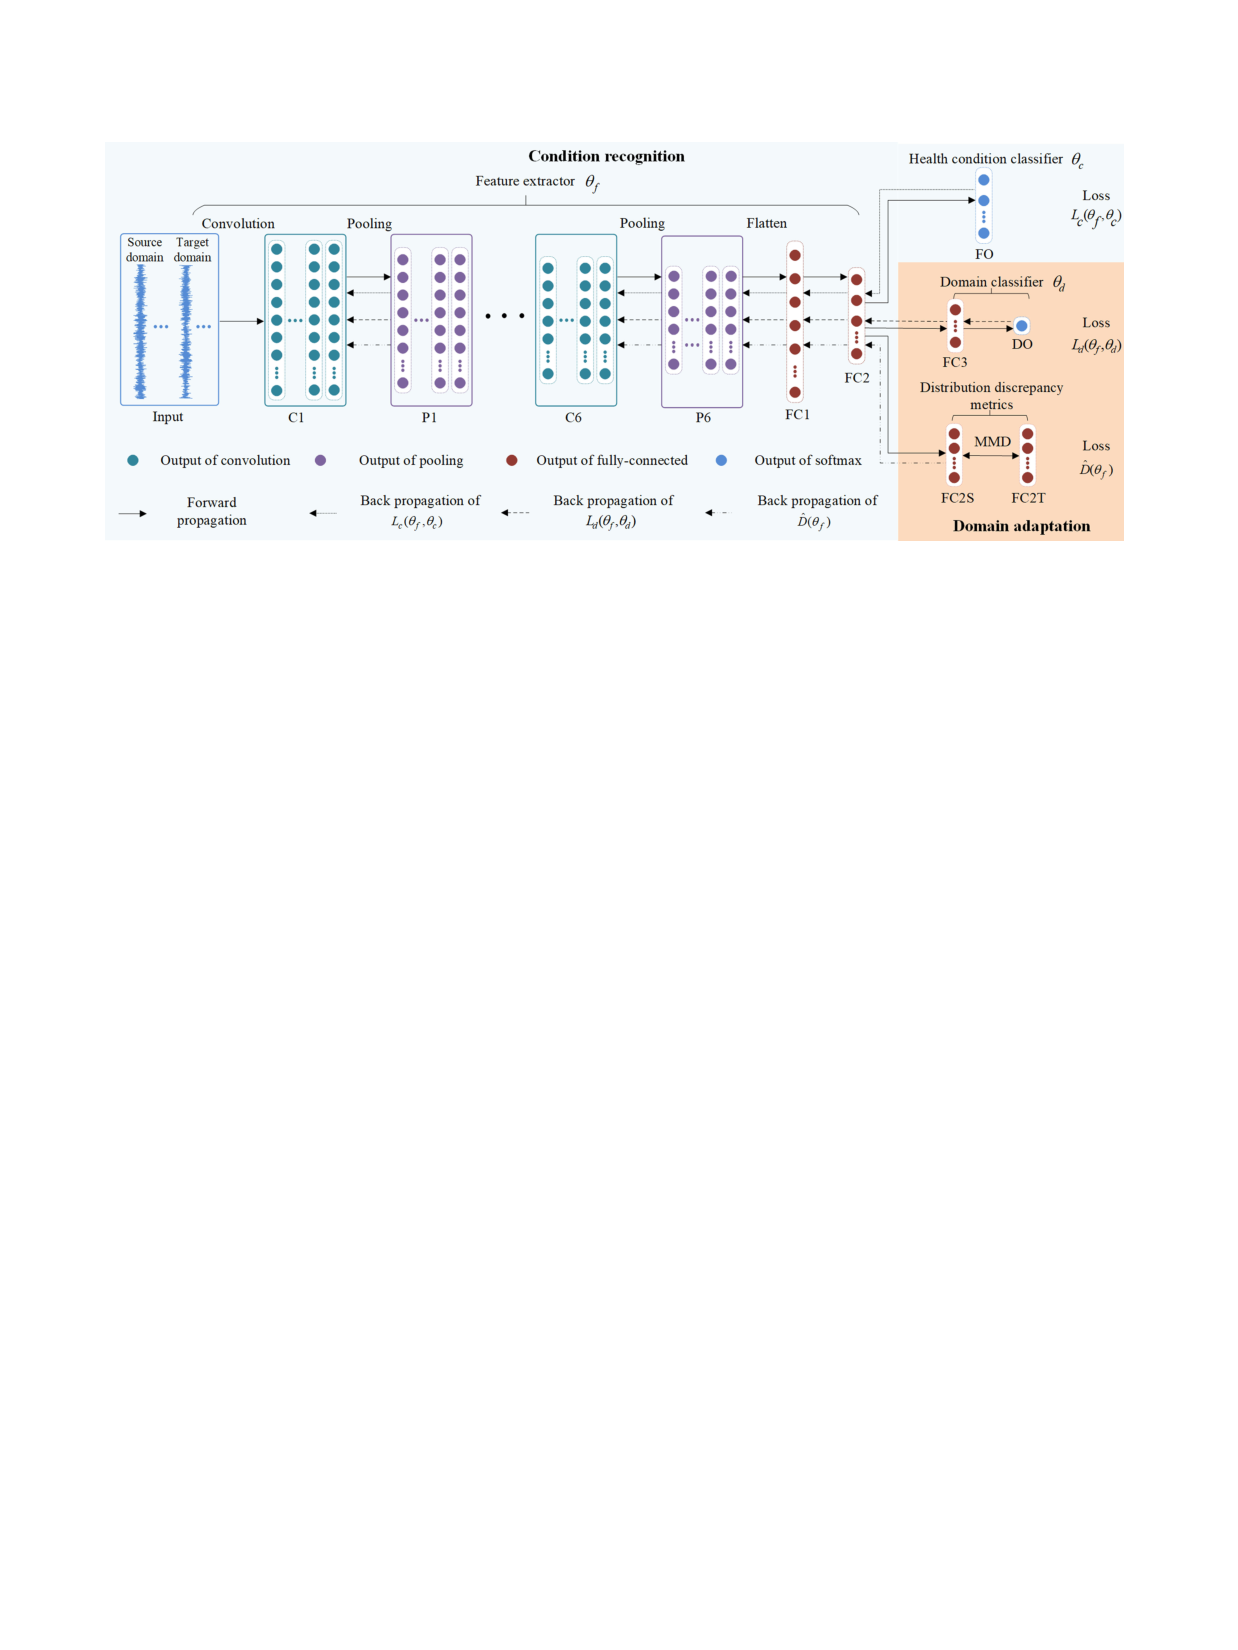
\includegraphics[width=1\textwidth]{models_state_of_the_art/DCTLN_model.pdf}
  \caption{DCTLN model proposed by Guo et al \cite{Guo2019}}
  \label{fig:DCTLN_model}
\end{figure}


\subsection{Wasserstein Distance Guided Multi-Adversarial Network for Prognostics and Healthmanagment for Rolling Bearings}
Zhang et al \cite{Zhang2019} present a Wasserstein distance guided multi-adversarial network (WDMAN) for rolling bearing fault diagnosis under different working conditions. The proposed architecture consists of a CNN feature mapper and a subsequent classifier. In the fully connected layers of the classifier, several Domain Critic Networks estimate the domain discrepancy by applying the Wasserstein-distance. A source CE-loss is applied in the end of the network. The whole model and the applied losses are visualized in fig. \ref{fig:WDMAN_model}.

 \begin{figure}[H]
  \centering
  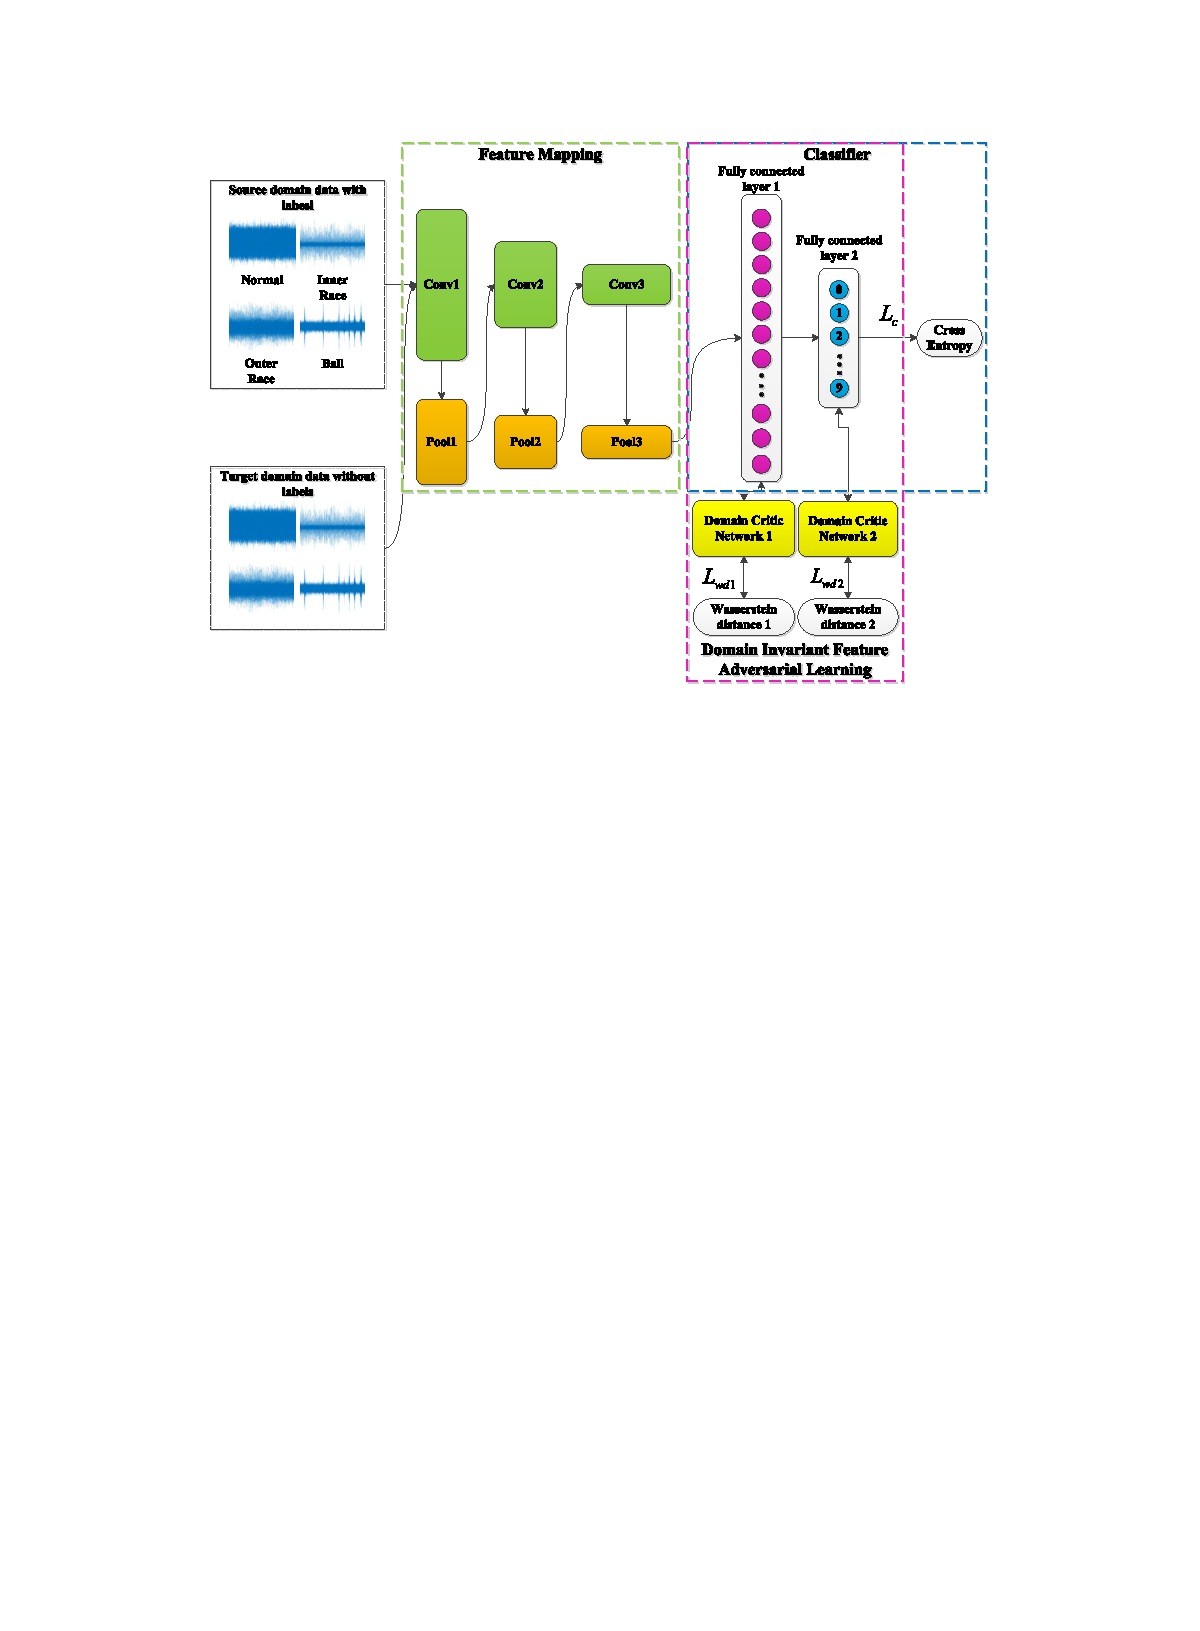
\includegraphics[width=1\textwidth]{models_state_of_the_art/WDMAN_model.pdf}
  \caption{WDMAN architecture proposed by Zhang et al \cite{Zhang2019}}
  \label{fig:WDMAN_model}
\end{figure}

In a pre-training phase, the feature mapper $\theta_{M}$ and classifier $\theta_{C}$ are optimized with the source CE-loss:
 
\begin{equation}
     L_{c}(x^{s}, x^{t}) = -\frac{1}{n^{s}} \sum_{i=1}^{n^{s}} \sum_{k=1}^{K} l(y_{i}^{s}=k) \cdot logC(M(x_{i}^{s}))_{k},
\end{equation}

where $n^{s}$ is the number of source samples, $K$ is the number of classes, $x_{i}^{s}$ and $y_{i}^{s}$ are the source samples and corresponding labels, $M(\cdot)$ and $C(\cdot)$ are the feature mapper and classifier. In the adversarial training afterwards, the model learns to extract more domain invariant features by minimizing the Wasserstein distance in the fully connected layers of the classifier. The domain critic networks try to maximize and the feature mapper to minimize the adversarial loss. The adversarial training transfers the model, trained on the source domain, to the target domain:
 
\begin{equation}
     L_{wd}(x^{s}, x^{t}) = \frac{1}{n^{s}} \sum_{x^{s} \in X^{s}} D(F(x^{s})) - \frac{1}{n^{t}} \sum_{x^{t} \in X^{t}} D(F(x^{t})),
\end{equation}

where $x^{s}$ and $x^{t}$ are the data samples drawn from the source domain $X^{s}$ and target domain $X^{t}$. The feature representations of the source and target samples in the fully connected layers are denoted as $F(\cdot)$. The domain critic networks are represented by $D(\cdot)$. In the adversarial learning, the model and discriminators are optimized in an alternating procedure:

\begin{equation}
    \min_{\theta_{F}} \max_{\theta_{D}} (L_{wd} - \lambda L_{gp}), 
\end{equation}

where $\theta_{F}$ and $\theta_{D}$ are the parameters of the feature mapper and domain critics, $\lambda$ is the penalty coefficient. Generally, the goal of the discriminators is to identify the domain of each sample. The feature mapper tries to extract domain-independent features, which precludes the discriminator predicting the correct domain. To satisfy the Lipschitz constraint condition of the Wasserstein distance, an additional gradient penalty is applied: 

\begin{equation}
     L_{gp}(\tilde{x}) = (|\nabla_{\tilde{x} \in P_{\tilde{x}}} D(\tilde{x})|_{2}-1)^{2}, 
\end{equation}
where $P_{\tilde{x}}$ is a distribution of samples coming from the line connecting a pair of points sampled from the source and target domain. The Wasserstein distance is extended with the gradient penalty. The workflow of the model is described more detailed in fig. \ref{fig:WDMAN_workflow}
 
\begin{figure}[H]
  \centering
  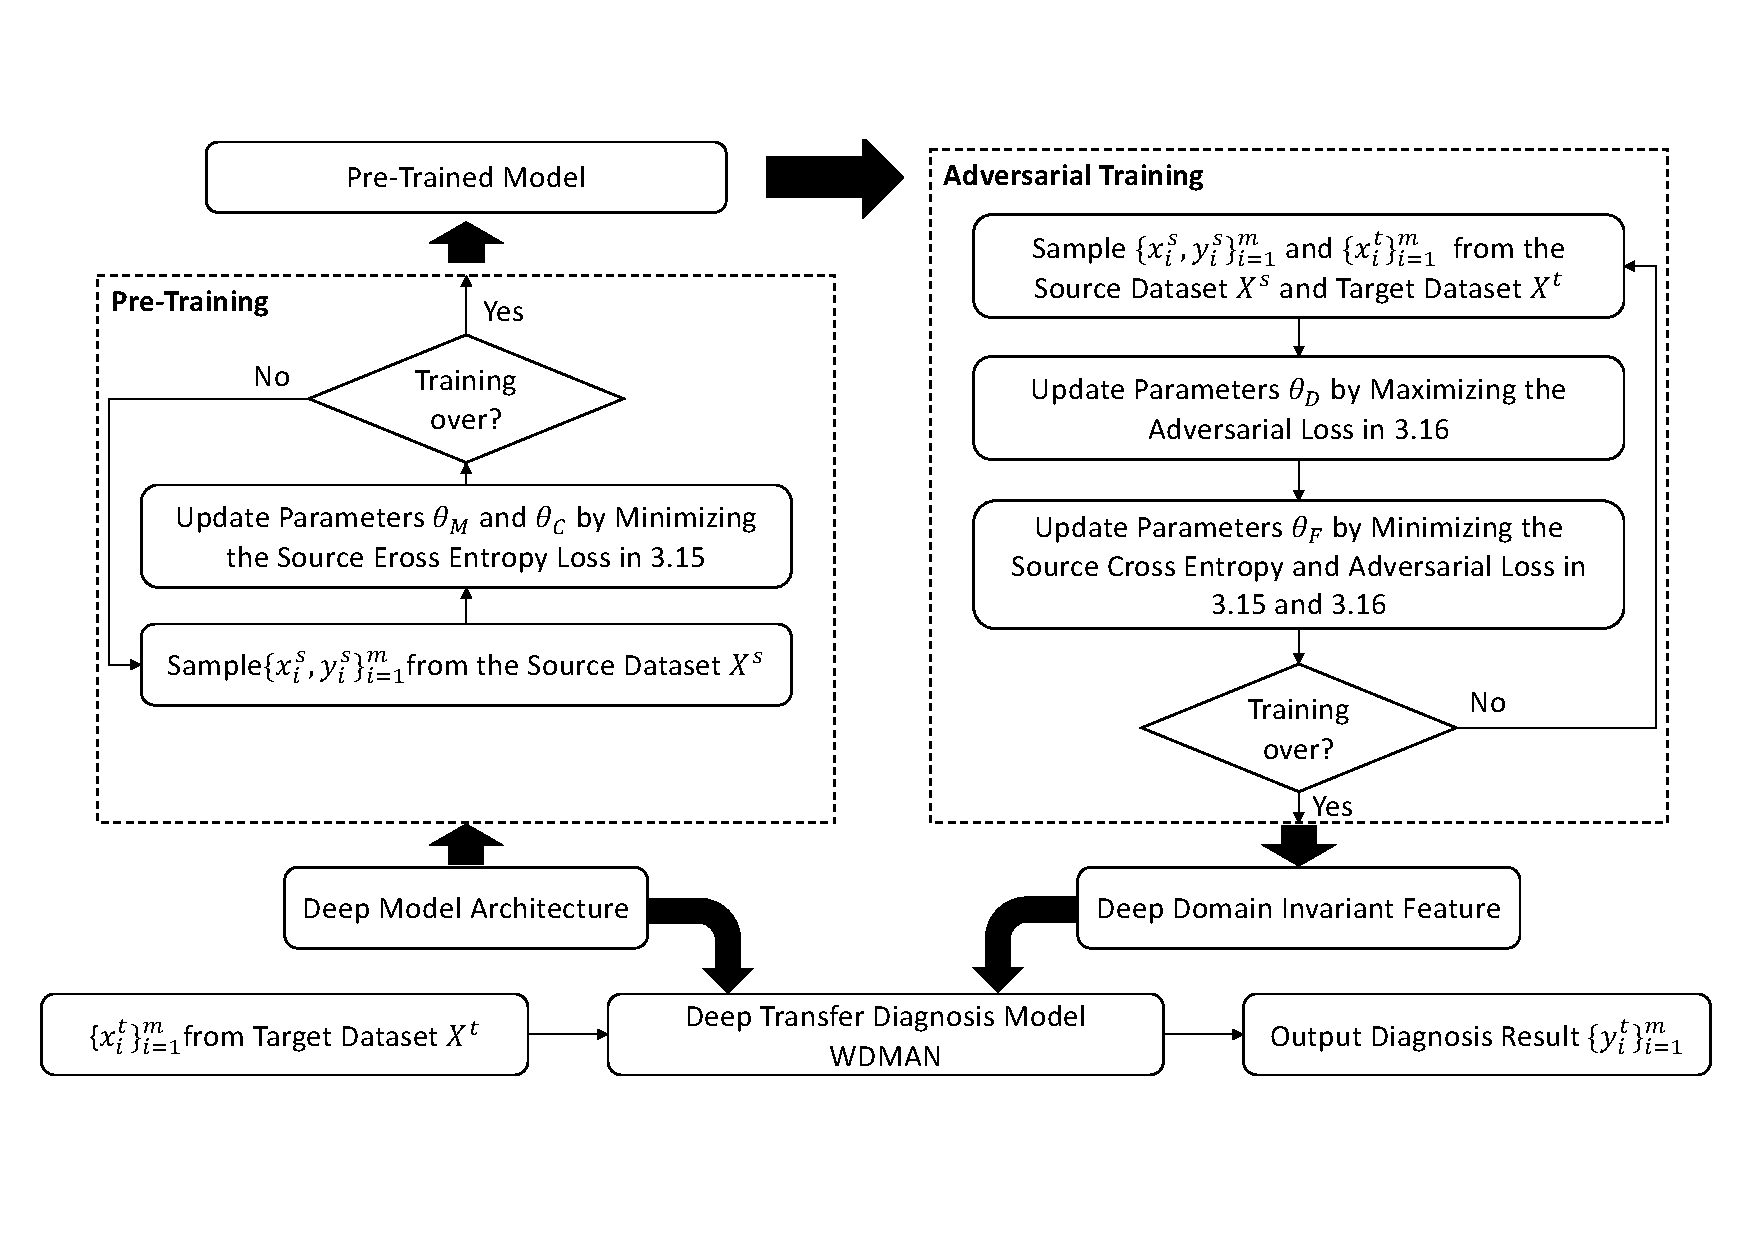
\includegraphics[width=.9\textwidth]{models_state_of_the_art/WDMAN_workflow.pdf}
  \caption{WDMAN workflow based on \cite{Zhang2019}}
  \label{fig:WDMAN_workflow}
\end{figure}
 
 
\subsection{Domain Conditioned Adaptation Network}
Most domain adaption approaches reduce the domain discrepancy in task-specific layers but use a shared feature extractor backbone across all domains. Li et al \cite{li2020} assume that, if the domain discrepancy is tremendously large, these methods can only reduce the domain discrepancy, but not fundamentally eliminate it. In the proposed Domain Conditioned Adaptation Network (DCAN) Li et al present some alternative and more effectively domain adaptive approach. Li et al recommend to extract domain-specific and -independent features in the feature extractor backbone. Since the source and target domains are correlated to some extend, the network itself can extract domain-independent features. The powerful feature extractor learned from the source domain can also increase the model performance on the target domain. At the same time, features which are too sensitive to the source domain can even reduce the model performance on the target domain. To counteract that phenomena, Li et al recommend to additionally extract domain-specific features in the convolutional layers. This can improve the cross-domain feature alignment in the task-specific layers. A domain conditioned feature correction module is applied to reduce the domain discrepancy in the extracted domain-specific and -independent features. Additionally, the model is optimized with a conventional supervised source and a newly proposed unsupervised target CE-loss defined as following:

\begin{equation}
    \min_{G} L_{s} = -\frac{1}{n_{t}} \sum_{j=1}^{n_{t}} \sum_{k=1}^{C_{n}} G^{(k)}(\pmb{x}_{tj})logG^{(k)}(\pmb{x}_{tj}),
\end{equation}
where $G(\cdot)$ is the learned predictive model, $n_{t}$ the number of source domain samples, $C_{n}$ the classes present in source and target domain and $\pmb{x}_{t}$ the target samples. The presented model is developed for computer vision applications and is never been evaluated in the context of PHM. Since PHM suffers from similar problems, this approach might be relevant and interesting for the PHM community. The model is visualized in fig. \ref{fig:DCAN_model}. In the following, the two domain adaption modules are described in more detail \cite{li2020}. 


\subsubsection{Domain Conditioned Channel Attention Mechanism}
Li et al \cite{li2020} use ResNet as backbone network, which allows an easy implementation of the domain conditioned channel attention module in its residual block. In the latent feature maps the processed images are represented as $\pmb{X}_{t} = [X^{1}_{t},...,X^{C}_{t}] \in \mathbb{R}^{HxWxC}$, where H and W are the spatial dimension and C the number of image channels. First, a channel-wise global average pooling layer is applied which reduces the images to  $\pmb{g}_{t} = [g^{1}_{t},...,g^{C}_{t}] \in \mathbb{R}^{1x1xC}$. Afterwards, the data is split depending on its domain and passed through different fully connected layers. The upper flow is used for target and the lower flow for source domain samples. The two different source and target domain routes share parameters. For both domains, an attention mechanism is trained jointly to learn activating different channels in the domain samples. This allows extracting more enriched domain specific features. In the fully connected layers the dimension is first reduced with a ratio ${1x1x\frac{C}{r}}$ and later reconstructed to its original size ${1x1xC}$. Relu and Sigmoid functions are applied. The domain-wise feature selection is achieved by weighting the channels of the feature representations $\pmb{X}_{s}$ and $\pmb{X}_{t}$ with the channel attention vectors $\pmb{v}_{s}$ and $\pmb{v}_{t}$ calculated by the domain conditioned channel attention module:

\begin{equation}
    \begin{aligned}
        &\pmb{\tilde{X}}_{s} = \pmb{v}_{s} \odot \pmb{X}_{s} = [v_{s}^{1} \cdot X_{s}^{1}, ..., v_{s}^{C} \cdot X_{s}^{C}]\\
        &\pmb{\tilde{X}}_{t} = \pmb{v}_{t} \odot \pmb{X}_{t} = [v_{t}^{1} \cdot X_{t}^{1}, ..., v_{t}^{C} \cdot X_{t}^{C}].
    \end{aligned}
\end{equation}

The domain conditioned channel attention module allows the model to independently learn the importance of each channel for the classification of source and target domain samples \cite{li2020}.


\subsubsection{Domain Conditioned Feature Correction}
A feature correction block is placed after each of the l task-specific layers to counteract the decreasing transferability in high-level features. At the feature correction blocks, the data simultaneously passes through the regular network and the feature correction block, which consist of FC and Relu blocks. The feature correction block estimates the domain discrepancy in the feature representation of the task-specific layer:
\begin{equation}
    \Delta H_{l}(x_{t}) = H_{l}(x_{s}) - H_{l}(x_{t}),
\end{equation}
where $H_{l}(x_{s})$ and $H_{l}(x_{t})$ are the feature representations of the source and target domain samples in the task-specific layer l and $\pmb{x}_{s}$ and $\pmb{x}_{t}$ the source and target domain samples. The feature representation of the target domain samples is corrected as following:
\begin{equation}
    \hat{H}_{l}(x_{t}) = H_{l}(x_{t}) + \Delta H_{l}(x_{t}).
\end{equation}


The discrepancy between the regular feature representation of source domain samples $H_{l}(x_{s})$ and the corrected feature representation of the target domain samples $\hat{H}_{l}(x_{t})$ is measured with a MMD-loss in several layers:

\begin{equation}
    L_{M}^{l} = |\frac{1}{n_s} \sum_{i=1}^{n_{s}} \phi(H_{l}(x_{si}) - \frac{1}{n_t} \sum_{i=1}^{n_{t}} \phi(\hat{H}_{l}(x_{ti}))|_{H_{\kappa}}^{2}, 
\end{equation}
where $H_{\kappa}$ is the reproducing kernel Hilbert space (RKHS), $\kappa$ the characteristic kernel and $\phi$ corresponding feature map. The number of source and target samples is defined by $n_{s}$ and $n_{t}$. Reducing the domain discrepancy improves the feature transferability, but also transfers noise and unimportant information between the domains. This destroys the structure of the source and target domain data and makes the classification task even more difficult. To avoid this over-transfer between source and target, the model is enforced to keep the source data constant when passing through the feature correction blocks. Since $\Delta H_{l}(x_{s}) \approx 0$ would prevent the cross-domain feature correction, another regularization term tackles that problem:
\begin{equation}
    L_{reg}^{l} = \sum_{k=1}^{C_{n}}|\frac{1}{n_{s}^{k}} \sum_{x_{si} \in S^{k}} \phi(H_{l}(x_{si})) - \frac{1}{|R|} \sum_{x_{sj} \in R} \phi(\hat{H}_{l}(x_{sj}))|_{Hk}^{2}, 
\end{equation}
where $R$ is a random subset of source domain samples and $S^{k}$ is the set of source domain samples belonging to class k \cite{li2020}.

\begin{figure}[H]
  \centering
  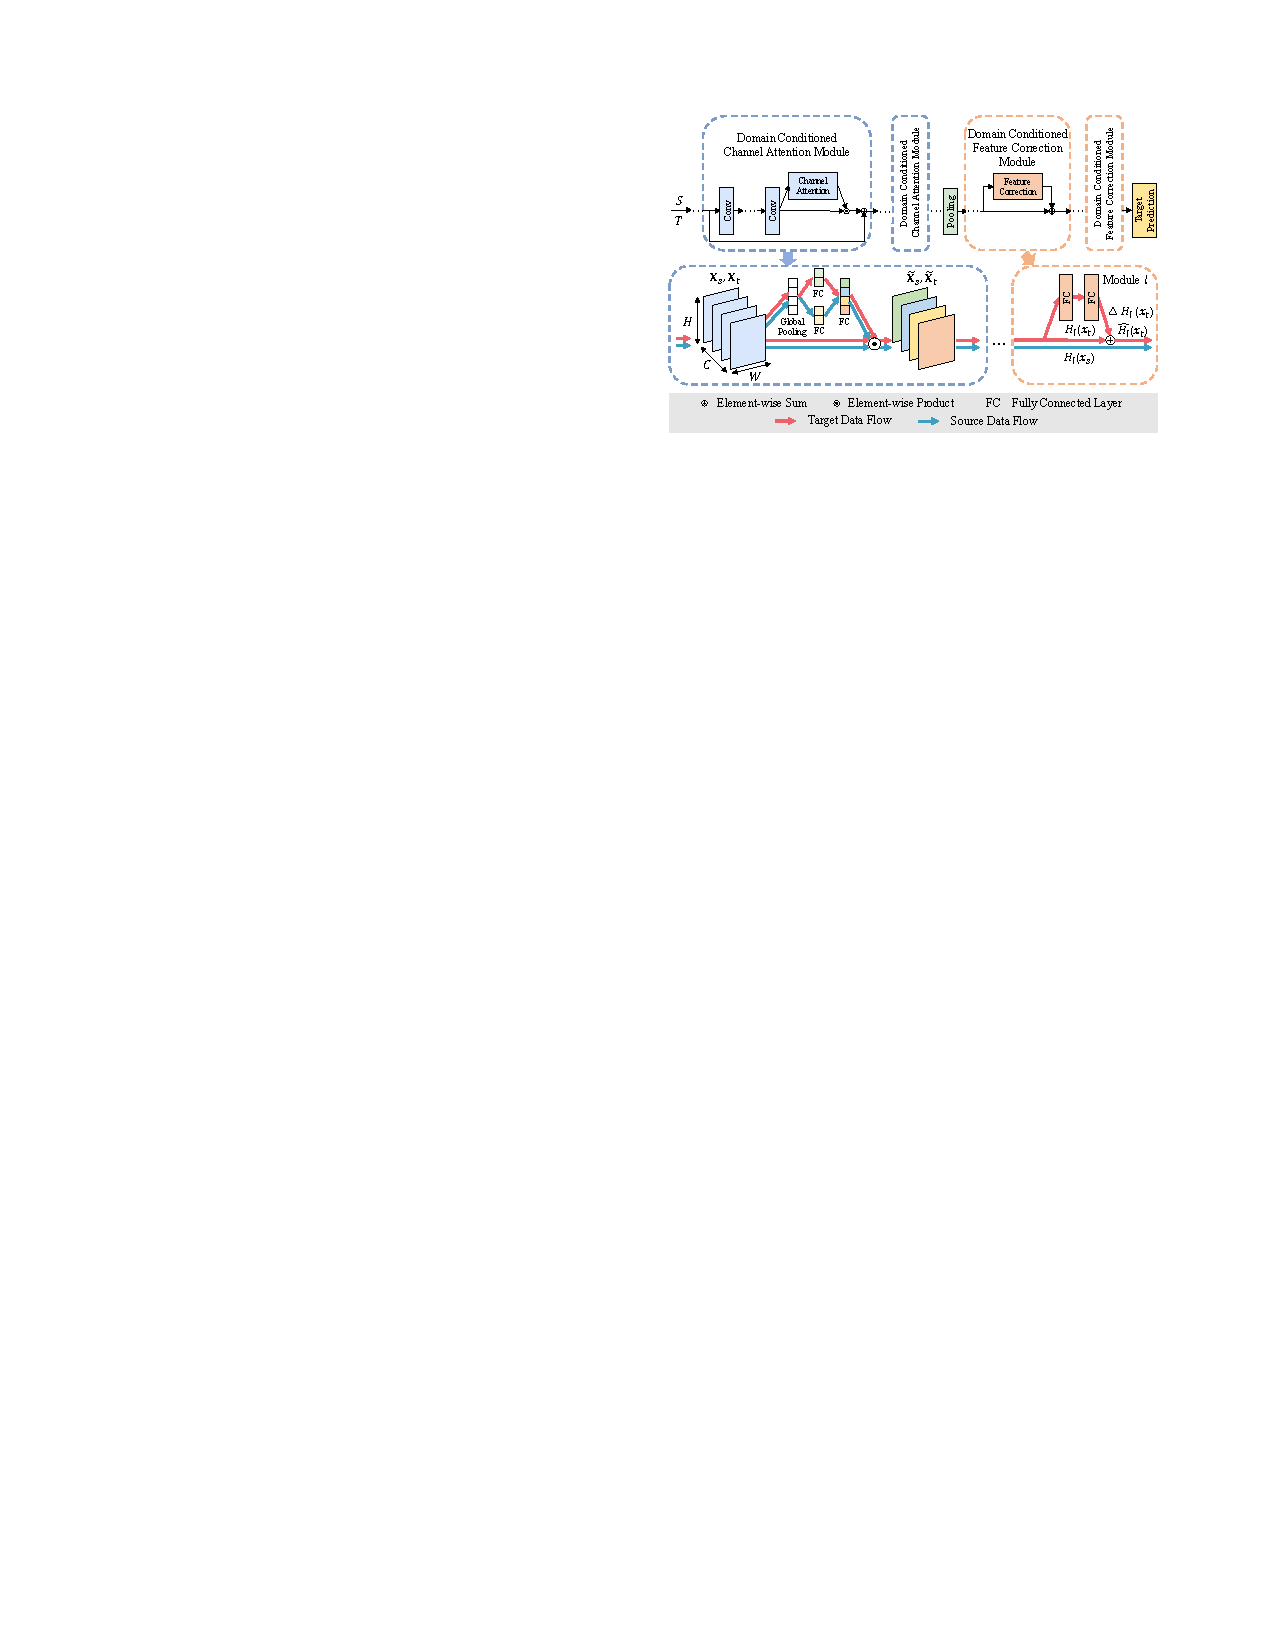
\includegraphics[width=1\textwidth]{models_state_of_the_art/DCAN_model.pdf}
  \caption{DCAN architecture proposed by Li et al \cite{li2020}}
  \label{fig:DCAN_model}
\end{figure}






Even sections are possible, but usually only used for several elements in, e.g.\ tables, images, etc.

\chapter{Figures}
\section{Example 1}
\cmark
\section{Example 2}
\xmark
\end{comment}